\documentclass{article}
\usepackage[utf8]{inputenc}
\usepackage{amsmath}
\usepackage{graphicx}

\title{Hello \LaTeX}
\author{Dark Lord}
\date{May 2020}

\begin{document}
\maketitle

Hello
% \section{Introduction}
\section*{Introduction}
Let's begin with a formula $e^{i\pi}+1=0$

% $$(1+\frac{1}{n})^n$$
% $$\left(1+\frac{1}{n}\right)^n$$

\begin{itemize}
\item But we can also do


\[
e = \lim_{n\to\infty}{\left(1+\frac{1}{n}\right)}^n = 
\lim_{n\to\infty} \frac{1}{ \sqrt[n]{n!}}   
\]

\item We can do another:

\[ 
    e = \sum_{n=0}^{\infty} \frac{1}{n!}
\]

\item We can use continued fractions

\[
    e = 2+\frac{1}{2+\frac{1}{2 + \frac{1}{\ddots}  }}
\]

\end{itemize}


\section*{More Formulas}

\[
    \int_{a}^{b} f(x)
\]

% The following \iiint control sequence is in package amsmath
\[
    \iiint f(x,y,z)
\]

\section*{Vectors}
\[
    \vec{v} = <v_1,v_2,v_3>
\]

\[
    \vec{v} \cdot \vec{w}
\]
% bmatrix
\[
    \begin{bmatrix}
        1 & 2 & 3 \\
        4 & 5 & 6 \\
        7 & 8 & 9 
    \end{bmatrix}
\]

\section*{Graphics}

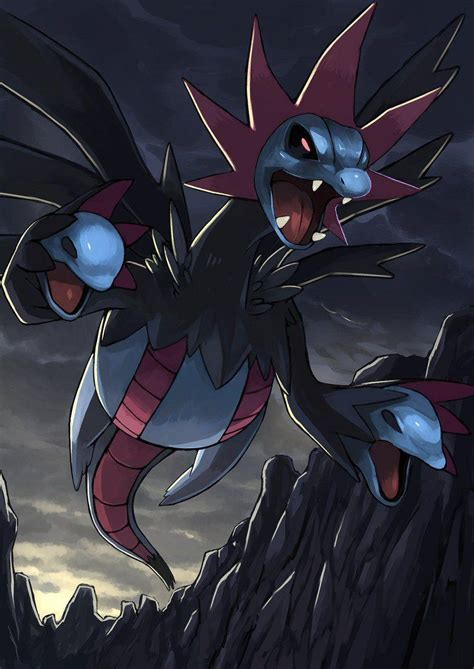
\includegraphics[scale=0.25]{img1}




\end{document}
